\documentclass[11pt,a4paper]{article}
\usepackage[a4paper,margin=2.3cm]{geometry}
\usepackage[T1]{fontenc}
\usepackage{lmodern}
\usepackage{microtype}
\usepackage{amsmath,amssymb}
\usepackage{graphicx}
\usepackage{float}
\usepackage{booktabs}
\usepackage{array}
\usepackage{enumitem}
\usepackage{caption}
\usepackage{xcolor}
\usepackage{titlesec}
\usepackage{fancyhdr}
\usepackage[hidelinks]{hyperref}

\definecolor{ivory}{HTML}{FBF8EF}
\definecolor{usopen}{HTML}{1D4F91}
\definecolor{clay}{HTML}{C65A2E}
\definecolor{ink}{HTML}{1E2633}

\titleformat{\section}{\Large\bfseries}{\thesection}{0.6em}{}
\titleformat{\subsection}{\large\bfseries}{\thesubsection}{0.6em}{}
\titlespacing*{\section}{0pt}{1.4em}{0.6em}
\captionsetup{font=small,labelfont=bf}
\setlist{itemsep=2pt,topsep=4pt}
\renewcommand{\arraystretch}{1.15}
\graphicspath{{../../report_assets/}}

\pagestyle{fancy}
\fancyhf{}
\renewcommand{\headrulewidth}{0pt}
\fancyfoot[L]{\small Queueing-Based Design of Airport Security Checkpoints}
\fancyfoot[R]{\small\thepage}

\newcommand{\Wq}{W_q}

\begin{document}

\begin{titlepage}
\centering
\vspace*{5cm}
{\Huge\bfseries Queueing-Based Design of\\[0.3em] Airport Security Checkpoints\par}
\vspace{1em}
{\Large MSL304 Course Project\par}
\vspace{3cm}
{\large Sohana Kumar (2024CS10251)\\ Sidharth Valsan (2024MT10433)\par}
\vspace{1em}
IIT Delhi \textperiodcentered{} November 2026
\vfill
{\small Live app: \href{https://msl304-security-queue-tool.streamlit.app/}{\nolinkurl{msl304-security-queue-tool.streamlit.app}}\\[0.3em]
Code: \href{https://github.com/sidoreon/msl304-security-queue-tool}{\nolinkurl{github.com/sidoreon/msl304-security-queue-tool}}\par}
\end{titlepage}

\section*{Summary}
We built a tool that tells a security checkpoint how many screening lanes to open in each 30-minute block and how to arrange the queue. Passengers are the customers and each lane is a server. The user enters arrival rates, the service rate of a lane and two costs; the tool returns lanes per block, the queue design and the saving against fixed all-day staffing. On an assumed test day (36 blocks, about 5{,}758 passengers, peak 11.79 passengers/min at 07:30):

\begin{itemize}
\item One shared queue cuts the mean wait by 59--93\% compared with a queue per lane, using the same lanes.
\item The cheapest plan uses 2 to 7 lanes and costs \textrm{INR}~60{,}090 a day, 42.6\% less than 6 lanes all day (\textrm{INR}~104{,}654).
\item A dedicated fast lane costs 19\% more per day and adds 0.24 min to every regular passenger's wait at the peak.
\item Another lane pays for itself once the open lanes are about 78--87\% busy.
\item Simulation agrees with every formula checked; bursty arrivals are the main risk.
\end{itemize}
All data and costs are assumed for illustration. The tool runs online at \href{https://msl304-security-queue-tool.streamlit.app/}{\nolinkurl{msl304-security-queue-tool.streamlit.app}}, and the code is at \href{https://github.com/sidoreon/msl304-security-queue-tool}{\nolinkurl{github.com/sidoreon/msl304-security-queue-tool}}.

\section{Problem}
Queues form when passengers arrive faster than the open lanes can screen them. Long waits cost passengers' time; extra lanes cost officers. The manager decides (i) the number of open lanes $c_t$ in each block $t=1,\dots,K$ and (ii) the queue design: one shared queue (\emph{pooled}), a queue per lane (\emph{separate}), or a priority lane. The goal is to minimise daily staffing plus waiting cost, subject to a waiting-time target in every block, utilisation below 1, and $1 \le c_t \le c_{\max}$.

\section{Models}
Arrivals are Poisson with rate $\lambda$ per minute, each lane serves at rate $\mu$, and the queue is first come, first served unless stated. Each block is treated as being in steady state.

\paragraph{Pooled queue (M/M/c).} With $a=\lambda/\mu$ and utilisation $\rho = \lambda/(c\mu)<1$,
\begin{align*}
P_0 &= \Bigl[\sum_{n=0}^{c-1}\frac{a^n}{n!} + \frac{a^c}{c!(1-\rho)}\Bigr]^{-1}, &
P_{\text{wait}} &= \frac{a^c}{c!(1-\rho)}P_0,\\
L_q &= P_{\text{wait}}\,\frac{\rho}{1-\rho}, \quad \Wq = \frac{L_q}{\lambda}, &
P(\Wq>t) &= P_{\text{wait}}\,e^{-(c\mu-\lambda)t}.
\end{align*}

\paragraph{Separate queues ($c\times$M/M/1).} Each passenger picks a lane at random, so each lane has $\lambda_i=\lambda/c$ and
\[
\Wq = \frac{\lambda_i}{\mu(\mu-\lambda_i)}, \qquad P(\Wq>t) = \frac{\lambda_i}{\mu}\,e^{-(\mu-\lambda_i)t}.
\]

\paragraph{Priority designs (M/G/1).} With $E[S_k^2]=(1+c_s^2)/\mu_k^2$ for class $k$ and share $p$ of priority passengers:
\begin{itemize}
\item \textbf{P1, fast lane}: one M/G/1 lane for priority passengers, $\Wq=\lambda_p E[S_p^2]/\bigl(2(1-\rho_p)\bigr)$; the other $c-1$ lanes form an M/M/$(c-1)$ queue for regular passengers.
\item \textbf{P2, priority in each lane}: non-preemptive priority, with $W_0=\sum_k \lambda_{k}E[S_k^2]/2$ per lane, $W_{q,1}=W_0/(1-\rho_1)$ and $W_{q,2}=W_0/\bigl((1-\rho_1)(1-\rho_1-\rho_2)\bigr)$.
\end{itemize}
For $c_s^2\ne1$ the pooled queue uses the Allen--Cunneen approximation $\Wq\approx\Wq(\text{M/M/}c)\,(1+c_s^2)/2$.

\section{Optimisation}
The cost of block $t$ with $c$ lanes is
\[
\text{cost}_t(c) = C_s\,c + C_w\,\lambda_t\,\Delta\,\Wq(c),
\]
where $\lambda_t\Delta$ is the number of passengers in a block of length $\Delta$. The problem is
\[
\min_{c_1,\dots,c_K}\ \sum_t \text{cost}_t(c_t) + C_{sw}\sum_t \max(0,\,c_t-c_{t-1})
\]
subject to $\Wq\le T$ (or $P(\Wq>T)\le\alpha$), $\rho_t<1$ and $1\le c_t\le c_{\max}$.

Without a switching cost ($C_{sw}=0$) the blocks are independent: the tool tries $c=1,\dots,c_{\max}$ in each block and keeps the cheapest feasible value. With a switching cost it solves the dynamic program $V_t(c)=\text{cost}_t(c)+\min_{c'}[V_{t-1}(c')+C_{sw}\max(0,c-c')]$, and checks the answer with an integer program in PuLP. Blocks that cannot meet the target run at $c_{\max}$ and are flagged. The baseline keeps the smallest number of lanes that meets the target at the peak open all day.

The break-even rate $\lambda^*$ for lane $c+1$ solves $C_w\lambda\Delta[\Wq(c;\lambda)-\Wq(c+1;\lambda)]=C_s$, found by a grid scan and Brent's method.

\section{The tool}
The tool is a Python package (\texttt{src/}) with a Streamlit app of six tabs: \emph{Problem}, \emph{Pooled vs Separate Queues}, \emph{Priority Lane Designs}, \emph{Staffing Plan}, \emph{Simulation Check} and \emph{Conclusions}. The first four tabs animate the checkpoint: lanes with an officer (black dot) at the top and passengers queueing below, with priority passengers as stars and the fast lane outlined (Figure~\ref{fig:app}). The plan downloads as CSV, and 98 automated tests cover the code.

\begin{figure}[H]
\centering
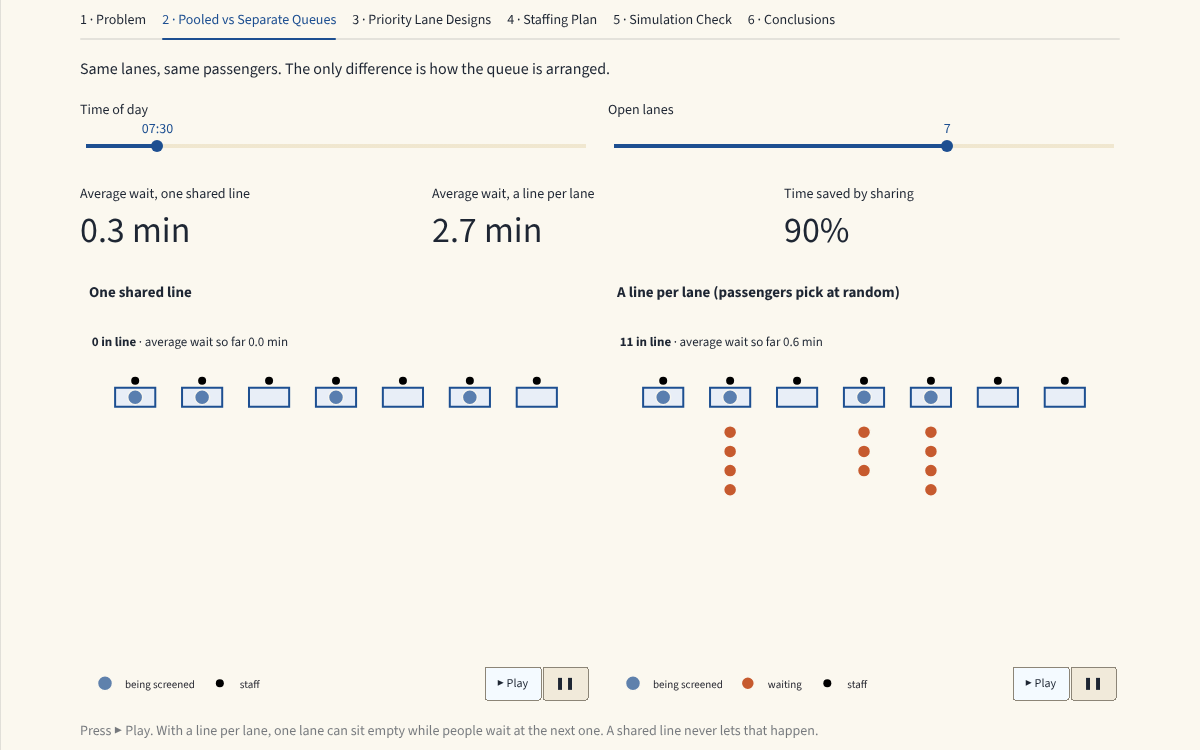
\includegraphics[width=0.72\linewidth]{screens/queues.png}
\caption{The same passengers at 07:30 with 7 lanes. Left: one shared line, nobody waiting. Right: a line per lane, 11 people waiting while two lanes stand empty.}
\label{fig:app}
\end{figure}

\section{Data}
The arrival profile is assumed: $\lambda(h)=2+10e^{-(h-8)^2/(2\cdot1.2^2)}+8e^{-(h-18)^2/(2\cdot1.5^2)}$ passengers/min for hour $h$, from 05:00 to 23:00. Defaults: $\Delta=30$ min, $\mu=2$/min, $c_s^2=1$, $c_{\max}=10$, $C_s=\text{INR }400$ per lane-block, $C_w=\text{INR }5$ per passenger-minute, $T=10$ min, $p=0.10$.

\section{Results}
\subsection{Pooling}
For the same lanes, the pooled queue cuts $\Wq$ by 59\% in quiet blocks and about 90\% at the peaks (Figure~\ref{fig:pool}); daily waiting falls from 8{,}960 to 1{,}298 passenger-minutes. Under the stricter target $P(\Wq>1\text{ min})\le0.10$, the peak needs 17 lanes with separate queues and 7 with a shared queue.

\begin{figure}[H]
\centering
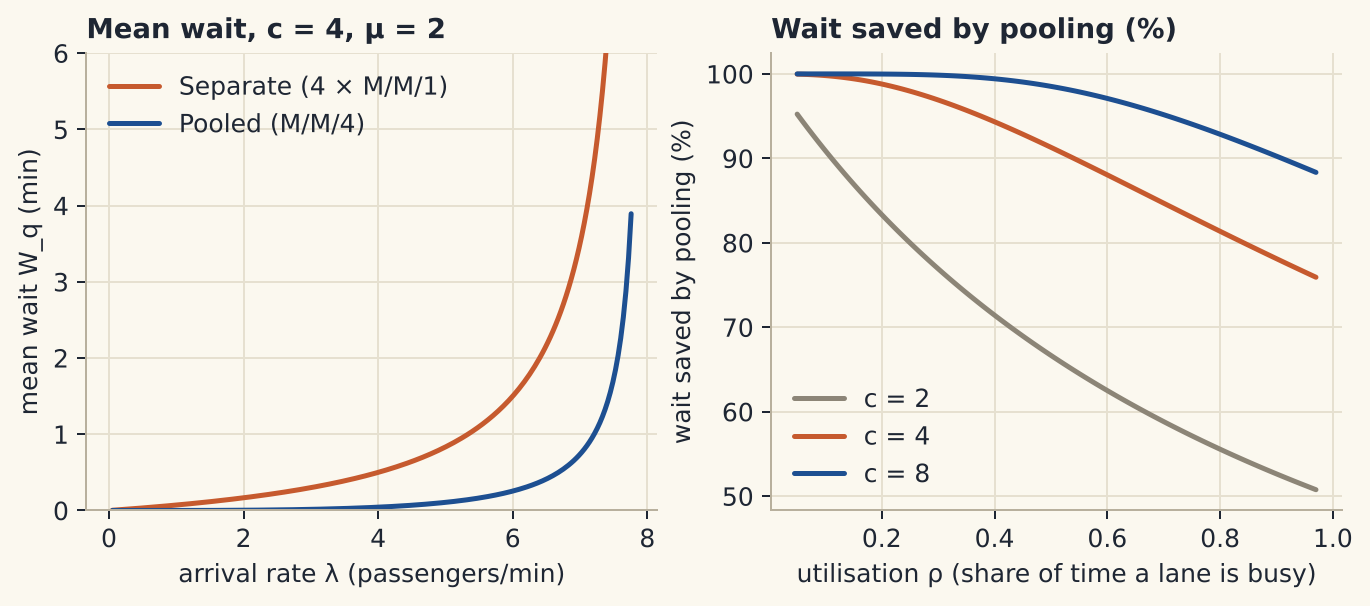
\includegraphics[width=0.92\linewidth]{fig_pooling.png}
\caption{Left: $\Wq$ against $\lambda$ for four lanes. Right: waiting removed by pooling.}
\label{fig:pool}
\end{figure}

\subsection{Staffing plan}
\begin{table}[H]
\centering
\begin{tabular}{lrrrr}
\toprule
Design & Optimised (INR) & Fixed baseline (INR) & Saving & Peak lanes\\
\midrule
\textbf{Pooled (M/M/c)} & \textbf{60,090} & 104,654 & 42.6\% & 7\\
Separate ($c\times$M/M/1) & 86,168 & 125,708 & 31.5\% & 10\\
P1 fast lane & 71,490 & 104,534 & 31.6\% & 8\\
P2 priority in each lane & 86,168 & 125,708 & 31.5\% & 10\\
\bottomrule
\end{tabular}
\caption{Daily cost of each design. The pooled queue is recommended.}
\end{table}

The recommended plan follows demand: 2 lanes at midday, 7 at the morning peak and 6 in the evening (Figure~\ref{fig:plan}). No block exceeds a mean wait of 0.46 min. At the peak, 6 lanes would meet the target, but a seventh lane costs INR 400 and saves about INR 7{,}360 of waiting, so the optimiser opens it. With a switching cost of INR 3{,}000 per lane opened, the plan keeps 3 lanes through midday instead; the dynamic program and integer program give the same cost.

\begin{figure}[H]
\centering
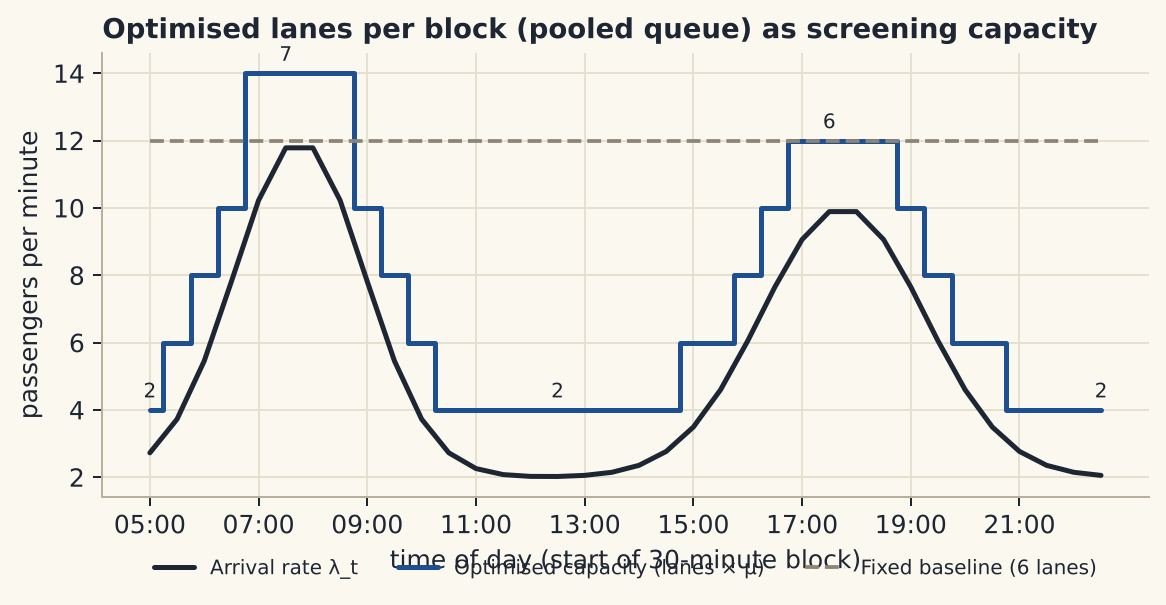
\includegraphics[width=0.85\linewidth]{fig_staffing.png}
\caption{Optimised capacity (lanes $\times\,\mu$) against arrivals and the fixed baseline.}
\label{fig:plan}
\end{figure}

\subsection{Priority lane}
At the peak ($\lambda=11.79$, $c=7$, $p=0.10$), P1 gives priority passengers 0.72 min and regular passengers 0.50 min, against 0.26 min for everyone in the plain pooled queue. P2 cuts the priority wait from 2.66 to 0.46 min but raises the regular wait to 2.90 min; the average is unchanged. With equal screening speeds, priority moves waiting between groups rather than reducing it.

\subsection{Break-even}
\begin{table}[H]
\centering
\begin{tabular}{lccccccccc}
\toprule
Step & 1$\to$2 & 2$\to$3 & 3$\to$4 & 4$\to$5 & 5$\to$6 & 6$\to$7 & 7$\to$8 & 8$\to$9 & 9$\to$10\\
\midrule
$\lambda^*$ & 1.56 & 3.22 & 4.93 & 6.68 & 8.44 & 10.22 & 12.02 & 13.83 & 15.65\\
Utilisation & 0.78 & 0.81 & 0.82 & 0.83 & 0.84 & 0.85 & 0.86 & 0.86 & 0.87\\
\bottomrule
\end{tabular}
\caption{Arrival rate above which one more lane pays for itself.}
\end{table}

\section{Simulation check}
A SimPy model (500 warm-up and 5{,}000 recorded passengers, 100 replications) was run for five blocks of the pooled plan and for all four designs at the peak. In all eight cases the formula value lies inside the 95\% confidence interval (Figure~\ref{fig:sim}). Stress tests at the peak show where the formulas break down:

\begin{table}[H]
\centering
\begin{tabular}{lr}
\toprule
Scenario & Mean wait (min)\\
\midrule
Poisson arrivals, all lanes open & 0.24\\
Groups of 3 on average & 1.06\\
Arrival rate alternating $\pm60\%$ & 7.37\\
One lane closed 25\% of each block & 0.37\\
Separate queues, random lane & 2.52\\
Separate queues, shortest lane & 0.34\\
\bottomrule
\end{tabular}
\caption{Stress tests at the morning peak (7 lanes).}
\end{table}

\begin{figure}[H]
\centering
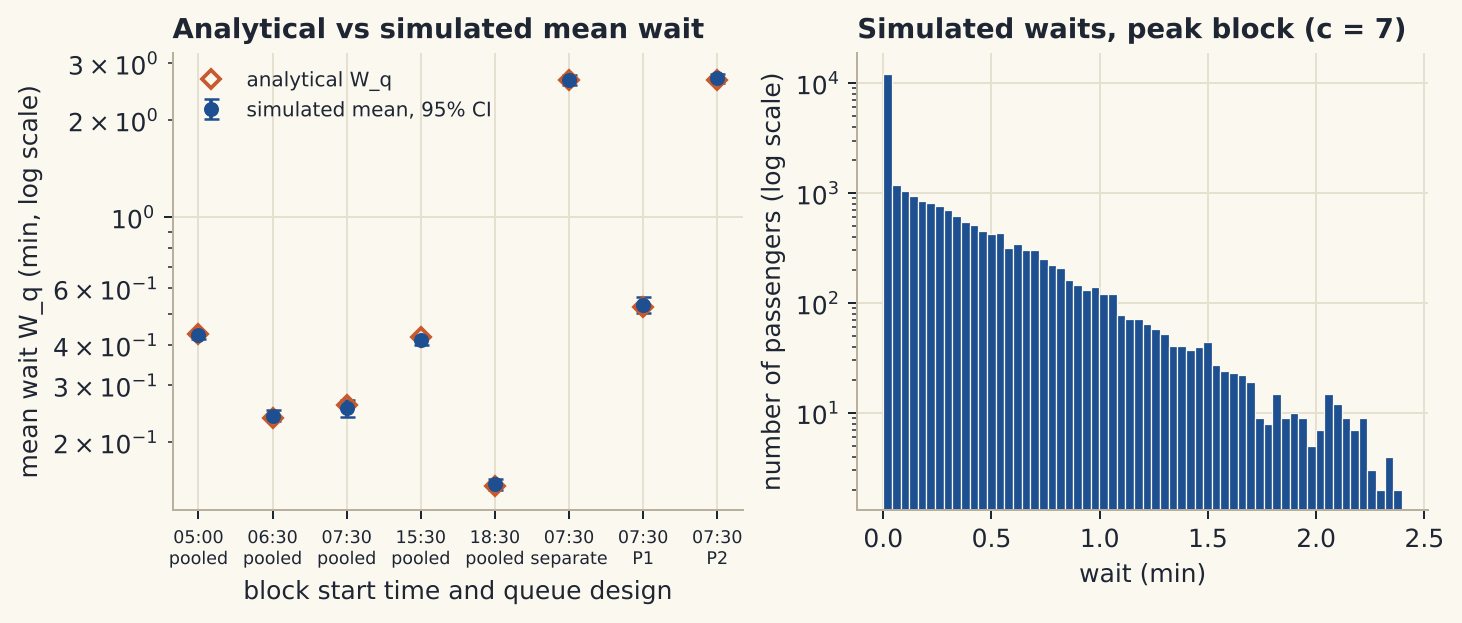
\includegraphics[width=0.78\linewidth]{fig_simulation.png}
\caption{Formula against simulation (left) and simulated waits at the peak (right).}
\label{fig:sim}
\end{figure}

\section{Sensitivity}
Varying one input at a time (Figure~\ref{fig:sens}), cost is most sensitive to the service rate ($\pm20\%$ moves it from INR 71{,}600 to 53{,}000) and the arrival level (51{,}200 to 69{,}500). The waiting target matters only when it is tight: at $T=10$ min it never binds.

\begin{figure}[H]
\centering
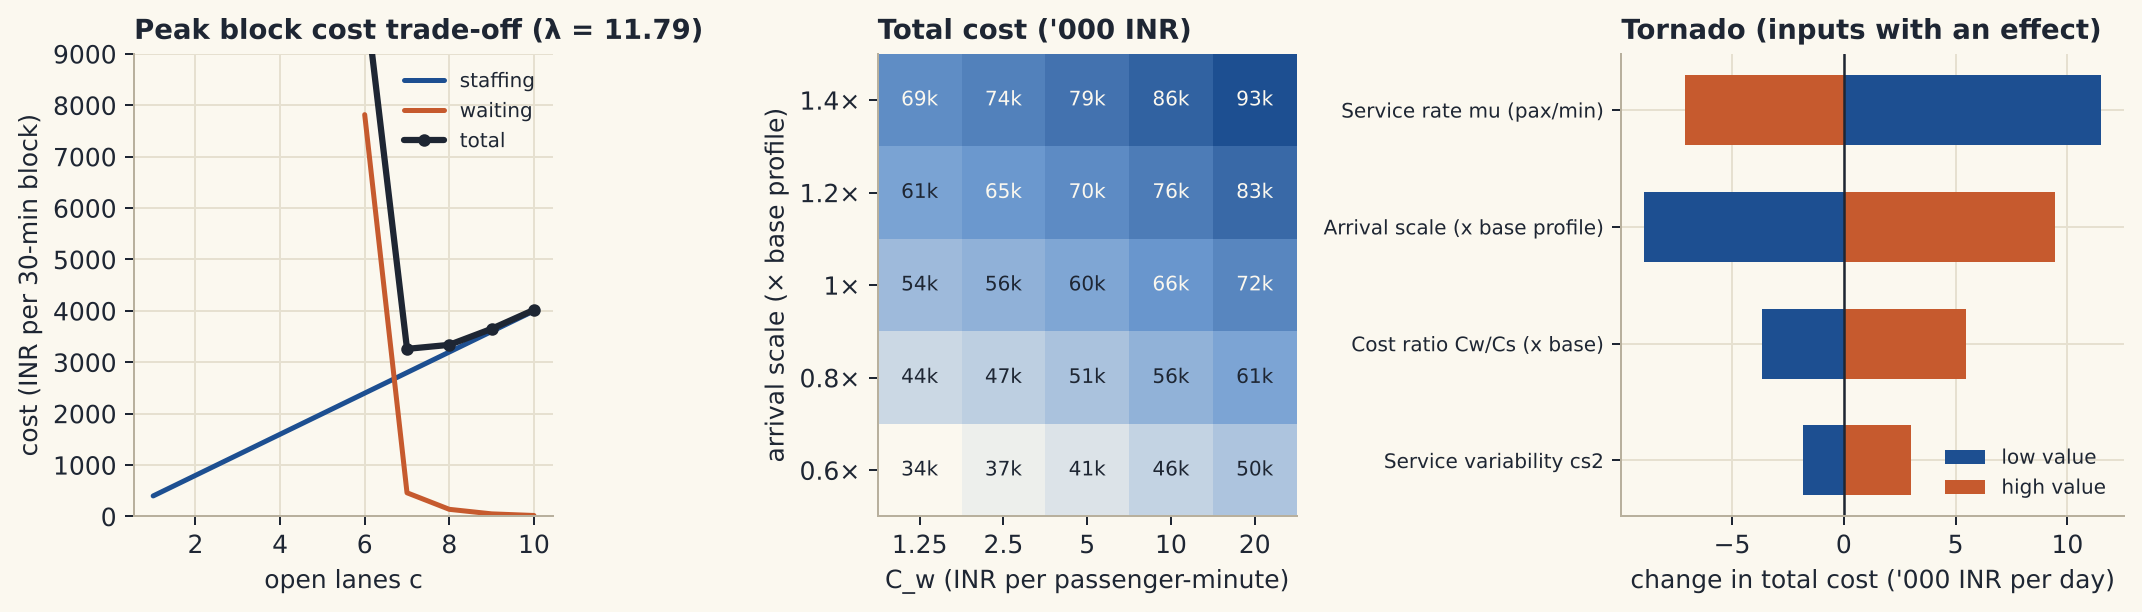
\includegraphics[width=0.88\linewidth]{fig_sens_tradeoff.png}
\caption{Peak-block cost against lanes, total cost by arrival scale and $C_w$, and the tornado chart.}
\label{fig:sens}
\end{figure}

\section{Contributions}
\textbf{Sidharth Valsan (2024MT10433), 55\%.} Wrote the code, including the Streamlit app and its queue animations, the lane optimiser and the automated tests. Generated the results and wrote them up, and recorded and edited the video.

\medskip\noindent\textbf{Sohana Kumar (2024CS10251), 45\%.} Built the queueing models for the shared line, separate lines and priority lanes, and set up the cost formulation. Ran the simulation check and the sensitivity and break-even analyses.

\medskip\noindent We planned the project and made the slides together, and both of us present in the video.

\section{Recommendations and limitations}
\begin{enumerate}[itemsep=1pt,topsep=3pt]
\item Use one shared line feeding all lanes.
\item Open and close lanes through the day to follow the arrival curve.
\item Open another lane when the open lanes are about 78--87\% busy.
\item Size any fast lane to the share of priority passengers.
\item Keep a spare lane for sudden rushes, which the Poisson model understates.
\end{enumerate}
The models assume steady state in each block, identical lanes and no abandonment, and all inputs should be replaced with measured data before use.

\end{document}
